
\section{Conclusions}
%Explain what conclusions you can draw from these set of experiments? The set of experiments and results reported here should justify some of the design choices described in the previous sections. (3-6 pages)
Figure  \ref{fig:exp-all-is} compares the Inception score for all tested network settings. Even though the Inception score of the basic DCGAN is not improved using the evaluated methods the overall quality of the generated images is clearly higher and the presence of mode collapse is significantly reduced or even non-existent for GAN's where spectral normalization, Wasserstein loss or both were added. In addition to these improvements both the D loss and G loss were much smoother during training. Having smoother losses allows for much better monitoring of the networks behavior during the training process leading to a much more intuitive hyper parameter tuning and debugging process. 
\begin{figure}[H]
\centering
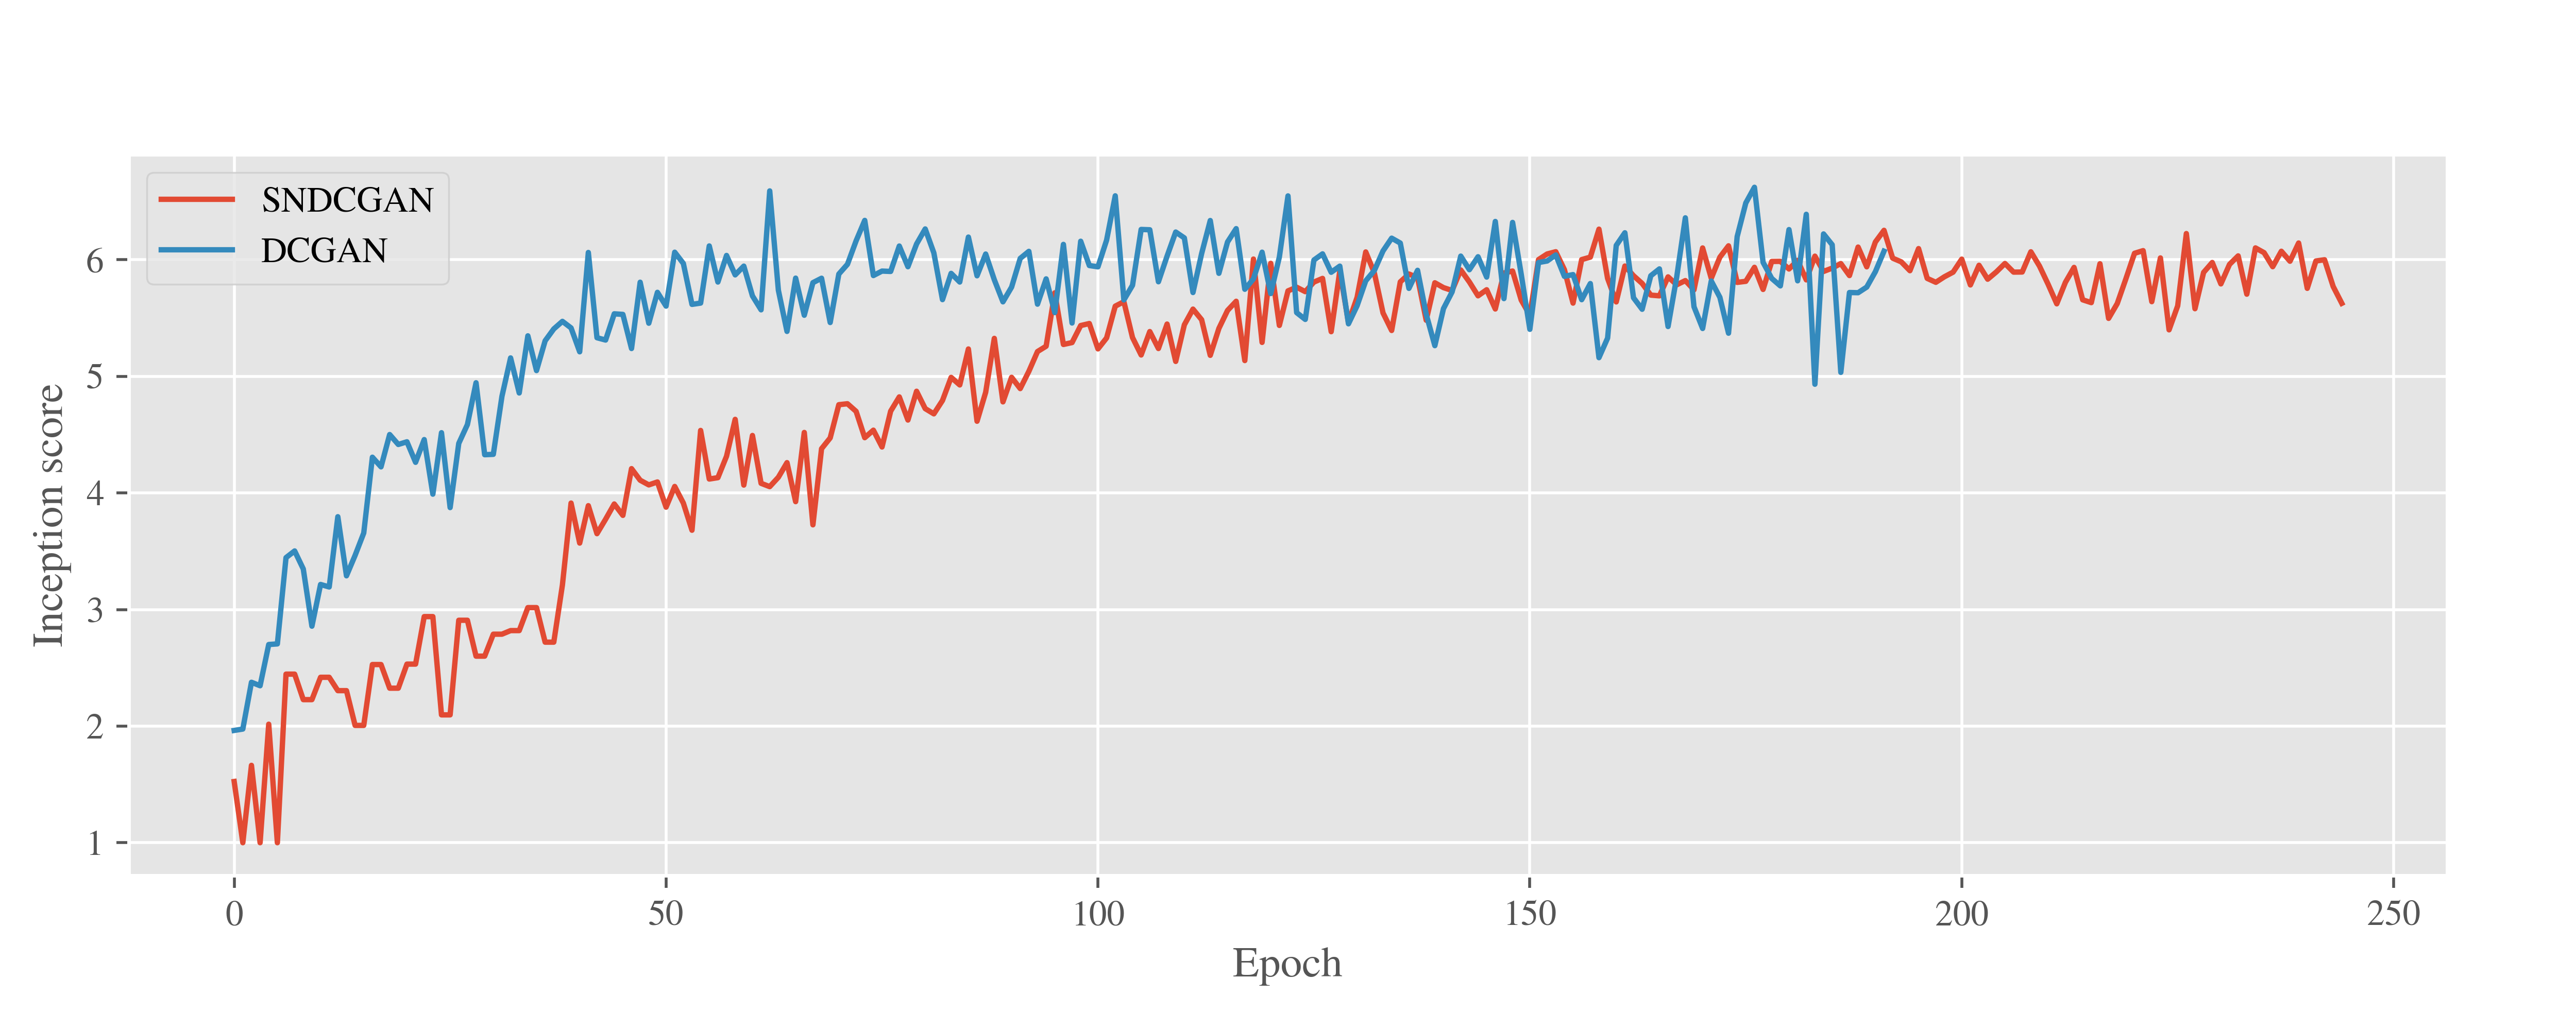
\includegraphics[width=\textwidth]{../code/results/figures/all_cifar10_is.png}
\caption{All evaluated models - Inception score, training on CIFAR10}
\label{fig:exp-all-is}
\end{figure}



%\todo{to justify the use of WGAN / the need for loss smoothness: Plotting these learning curves is not only useful for debugging and hyperparameter searches, but also correlate remarkably well with the observed sample quality. (taken from WGAN paper) }

\subsection{Future Work}


- LSGAN
- Gradient penalty
- Parameter search